% !TEX encoding = UTF-8 Unicode
%\documentclass{article}
%\usepackage{superstyle}

%\begin{document}
%oppgavetekst
Now remove the sinusoidal load and add a 70 kg diver to the beam, balancing on the last 20 cm of the beam. You must add a force per unit length of −g times 70/0.2 kg/m to f (xi ) for all 1.8 ≤ xi ≤ 2, and solve the problem again with the optimal value of n found in Step 5. Plot the solution and find the deflection of the diving board at the free end.

\vspace{5mm}
Løsning

\begin{lstlisting}[caption={Oppgave6regning.m}]
function [B] = Oppgave6Regning(n)
%deler først opp bjelken i n lengder med lengde h 
h = 2 / n;        

%Definerer konstanter. Lengden av planken = 2. g, d, w og t er konstanter i oppgaven. 
L=2;
g=9.81; 
d=480; 
w=0.3;
t=0.03; 

%regner ut kraften f(x) 
kraft = -d*w*t*g; 

%definerer E og I som gitt i oppgaven
E = 1.3*10.^(10); 
I = (w*t.^3)/12; 

%Lager en matrise B med høyde n og bredde 1. 
B = ones(n, 1);

%looper igjennom n
for k=1:n
	%definerer xi for hvert steg ut på brettet
    xi=k*h; 

    %Hvis vi befinner oss på slutten av planken (x mellom 1.8 og 2) er kraften annerledes. (gitt i oppgaven, vekten av stuperen)
    if xi>=1.8
        B(k, 1)=kraft-g*(70/0.2);

    %Hvis ikke er kraften som vanlig:
    else
        B(k, 1)=kraft;
    end
end;

%Til slutt ganger vi hele matrisen med h^4/(E*I)
B=B*h^4/(E*I);
\end{lstlisting}

Vi bruker denne koden til å få den vertikale forskyvningen på slutten av brettet, og lager en graf av brettets vertikale forskyvning:\\

\begin{lstlisting}[caption={Oppgave6.m}]
%Regner matrisen A med alle vertikale forskyvninger langs stupebrettet. Den
%optimale n funnet i forrige oppgave er 1280.
A=Oppgave6Regning(1280); 

%Definerer matrisen B på samme måte som før
B= lagmatrise(1280); 

%Regner ut C, som vil inneholde den vertikale forskyvningen til hvert punkt
%langs stupebrettet. (C=A*Binvers)
C=B\A; 

%Skriver ut den siste vertikale forskyvningen, altså forskyvningen på
%slutten av brettet. 
disp('Vertikal forskyvning på slutten av stupebrettet: '); 
disp(C(1280)); 

%Lager en x-vektor med x-verdier
x=0:(2/1280):(2-2/1280); 

%Lager en graf av x-verdiene og den vertikale forskyvningen
plot(x',C);
\end{lstlisting} 

Den vertikale forskyvningen på slutten av planken er $C(1280)=-0.2034$

\begin{figure}[h]
    \centering
    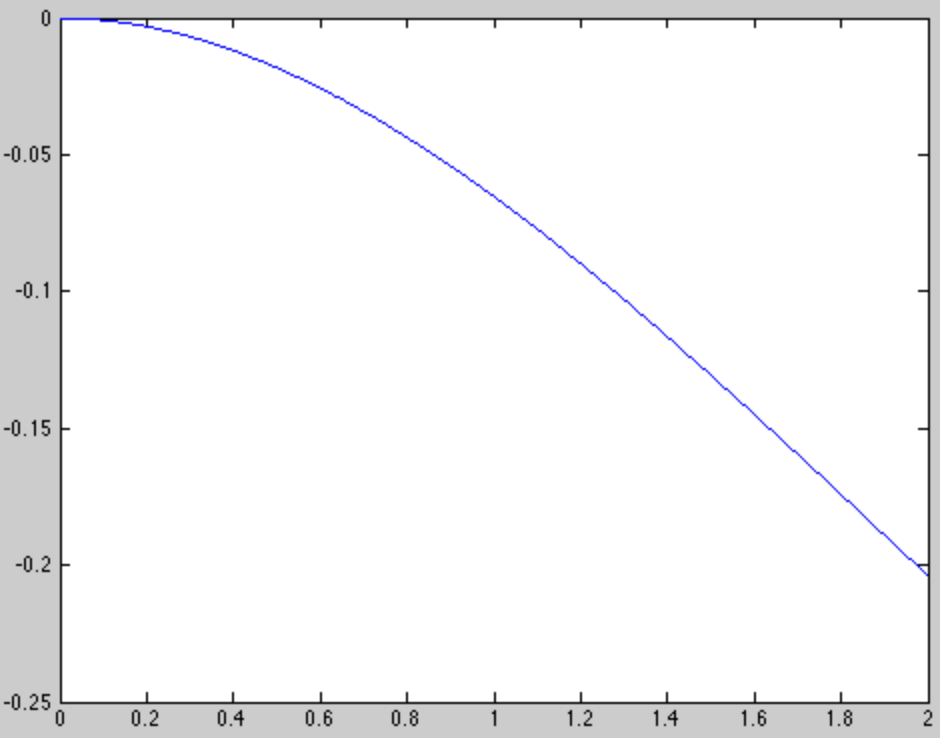
\includegraphics[width=0.8\textwidth]{sections/Exercise6/DiverGraph}
    % 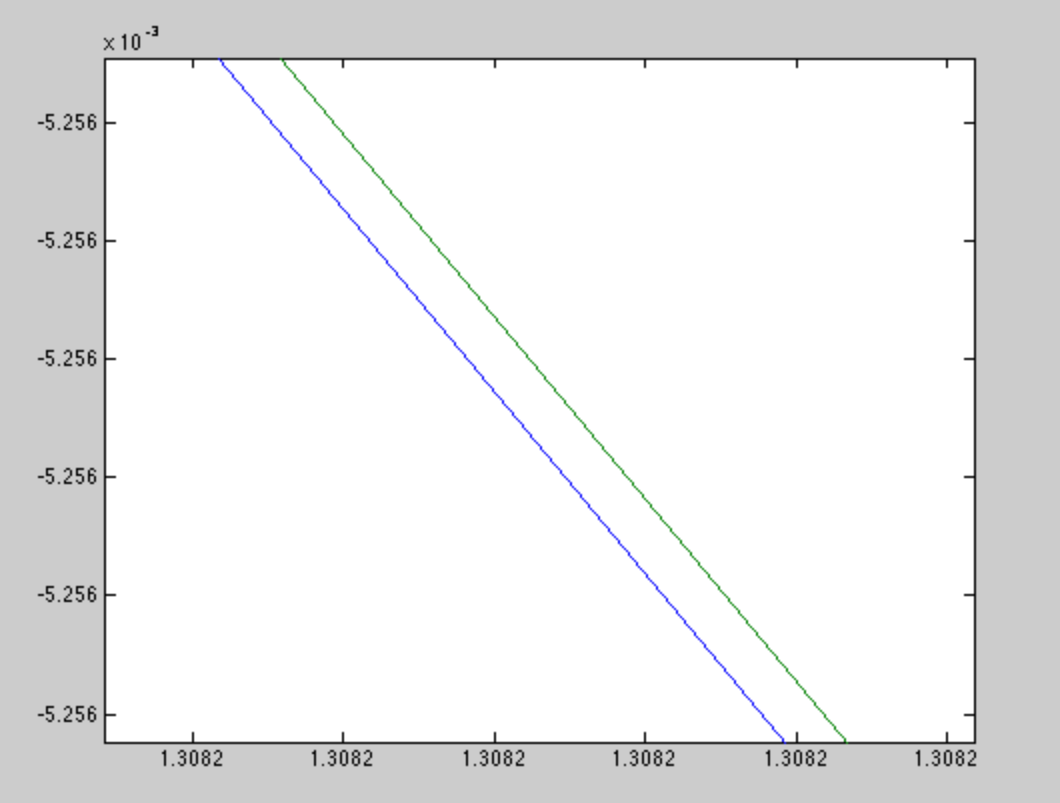
\includegraphics[width=0.8\textwidth]{errorplot2}
    \caption{Grafen til stupebrettet påvirket av stuperens vekt}
    \label{fig:divergraph}
\end{figure}

%\end{document}